原生 Word 样式验收样例（非正式论文）

摘要

本文件仅用于检查排版。示例中的 \textbf{10 μm} 与 \textbf{相位反演}
为强调样例，不构成新的研究结果。\emph{斜体}用于内容性强调。

关键词

原生样式；题注；可编辑公式

模型与符号

行内公式 \(y=ax+b\) 应保持可编辑。

\[
\delta(\nu)=4\pi t\nu\sqrt{n^2-\sin^2\theta}.
\]

符号说明（排版样例）

\begin{longtable}[]{@{}lll@{}}
\toprule\noalign{}
符号 & 含义 & 单位 \\
\midrule\noalign{}
\endhead
\bottomrule\noalign{}
\endlastfoot
\(t\) & 厚度 & μm \\
\(\nu\) & 波数 & cm⁻¹ \\
\end{longtable}

如 表1 所示，表题应在表上方。

检查层级

\begin{enumerate}
\def\labelenumi{\arabic{enumi}.}
\tightlist
\item
  检查标题编号。
\item
  检查列表编号。

  \begin{itemize}
  \tightlist
  \item
    检查嵌套列表。
  \end{itemize}
\end{enumerate}

图形展示

\pandocbounded{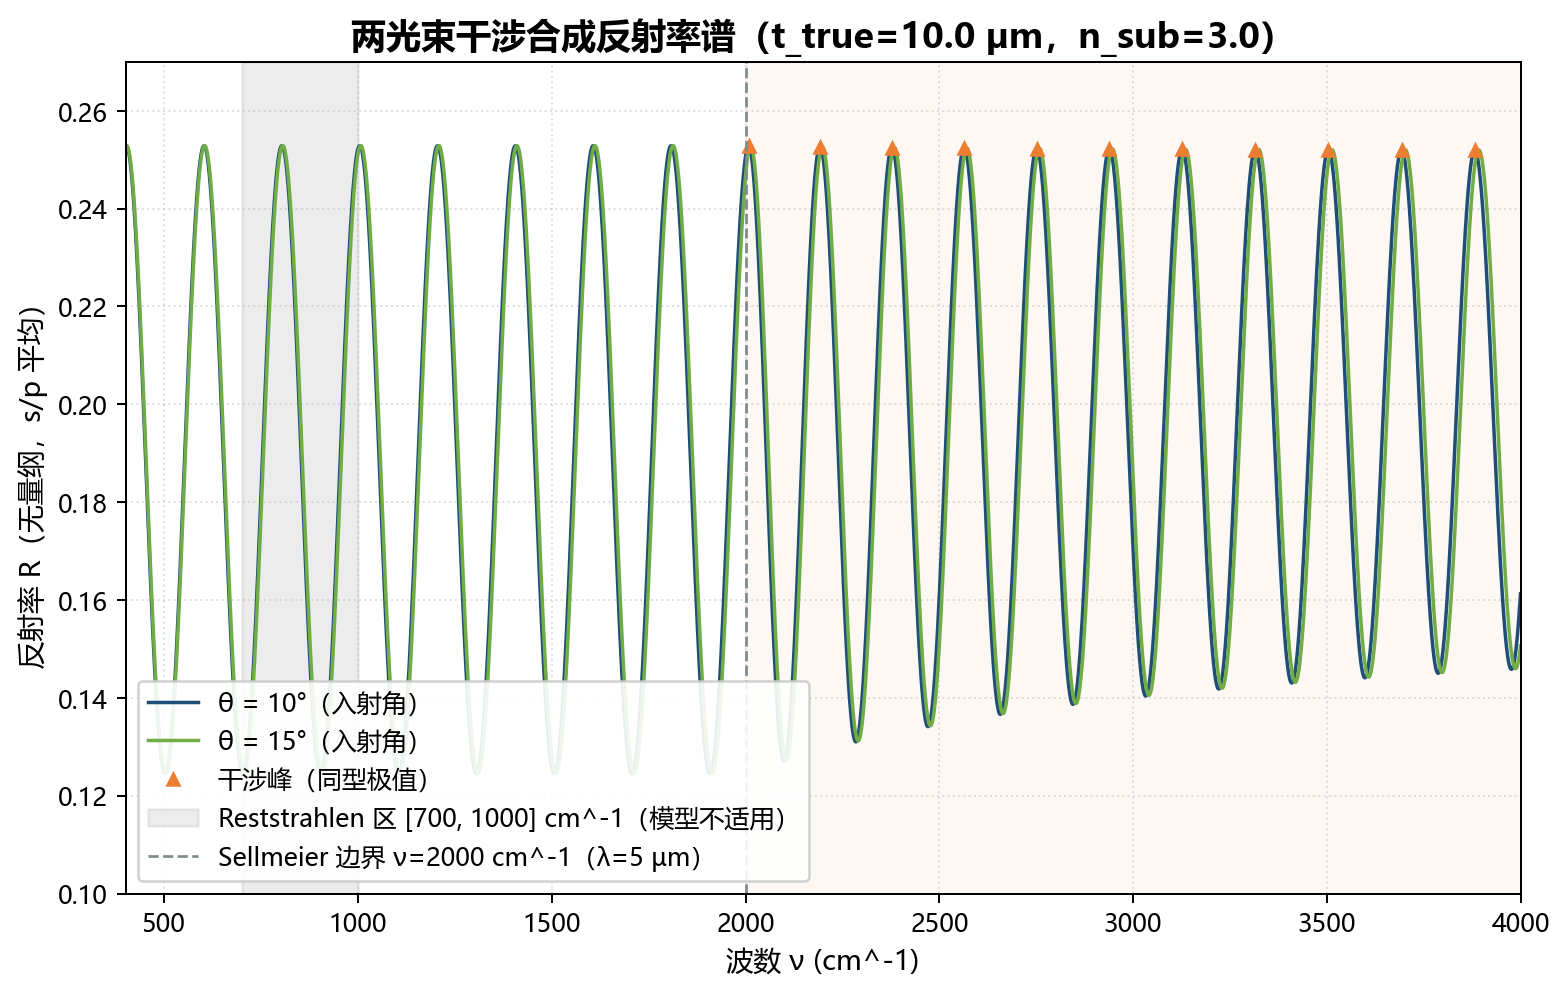
\includegraphics[keepaspectratio,alt={已验收合成反射率谱（仅用于图片排版检查）}]{problems/2025-cumcm-b/prob01/versions/assumption_v001/figures/prob01_fig_reflectance_spectrum_1d4fb899d1.png}}

已验收合成反射率谱（仅用于图片排版检查）

图1 展示已有合成谱图片，图下注明标题，不将图像检查日志写入正文。

参考文献

本样例不引入研究文献。

附录：验收说明

该文档不替代正式论文，不运行模型计算。
